\chapter{Johdato}
\label{cha:euler}

Leonhard Euler (1707--1783) oli sveitsiläinen matemaatikko ja fyysikko, joka on saanut nimensä niin matematiikan kuin tietojenkäsittelytieteenkin historiaan. Tässä luvussa esitellään muutama Eulerin kuuluisa saavutus.

\chapter{Eulerin identiteetti}
\label{cha:eulerin-identiteetti}

\emph{Eulerin identiteetti} on seuraava yhtälö:
\begin{equation}
  \label{eq:euler_id}
  \e^{i\pi}+1=0\; .
\end{equation}
Identiteettiä \eqref{eq:euler_id} kutsutaan usein \enquote{matematiikan kauneimmaksi kaavaksi} \citep{reid06zero}. Se sisältää viisi tärkeää lukua: $0$:n, $1$:n, $\e$:n, $i$:n ja $\pi$:n. Näistä kolme viimeisintä on määritelty taulukossa~\ref{tab:vakiot}. 

\begin{table}
  \centering
    \caption{Tärkeitä matematiikan vakioita}
  \label{tab:vakiot}
  \begin{tabular}{@{}Lp{0.5\textwidth}R@{}}
    \toprule
    \text{symboli} & merkitys & \text{arvo}\\
    \midrule
    \e & Neperin luku, $\lim_{n\to\infty}(1+1/n)^n$ & \approx 0{,}577 \\
    \pi & ympyrän kehän ja halkaisijan suhde & \approx 3{,}142 \\
    i & imaginaariyksikkö & \sqrt{-1} \\
    \bottomrule
  \end{tabular}
\end{table}

Eulerin identiteetti seuraa Eulerin yhtälöstä.

\begin{theorem}[Eulerin yhtälö]
  \label{thm:euler_thm}
  Kaikille $x\in\R$ pätee, että
  \begin{equation}
    \label{eq:euler_thm}
    \e^{ix}= \cos x + i \sin x\; .
  \end{equation}
\end{theorem}

\begin{proof}
  Eulerin yhtälön todistus perustuu Taylorin sarjoihin. Eksponenttifunktion $\e^x$, sinifunktion $\sin x$ ja kosinifunktion $\cos x$ sarjaesitykset ovat
  \begin{align}
    \e^x &= 1 + x + \frac{x^2}{2!} + \frac{x^3}{3!} + \cdots \label{eq:exp_taylor}  \\
    \sin x &= x - \frac{x^3}{3!} + \frac{x^5}{5!} - \frac{x^7}{7!} + \cdots \label{eq:sin_taylor} \\
    \cos x &= 1 - \frac{x^2}{2!} + \frac{x^4}{4!} - \frac{x^6}{6!} + \cdots \label{eq:cos_taylor} \; ,
  \end{align}
  missä $x\in \R$. Kompleksiluvulle $z\in\mathbb{C}$ vastaavat sarjat saadaan korvaamalla $x$ muuttujalla $iz$. Näin sijoittamalla saadaan
  \[
    \begin{split}
      \e^{iz} &= 1 + iz + \frac{(iz)^2}{2!} + \frac{(iz)^3}{3!} + \frac{(iz)^4}{4!} + \cdots \\
      & =1 + iz - \frac{z^2}{2!} - \frac{iz^3}{3!} + \frac{z^4}{4!} + \frac{iz^5}{5!} - \frac{z^6}{6!} - \frac{iz^7}{7!} + \frac{z^8}{8!} + \cdots \\
      &= \left(1 - \frac{z^2}{2!} + \frac{z^4}{4!} - \frac{z^6}{6!} + \frac{z^8}{8!} + \cdots\right)
      + i\left(z - \frac{z^3}{3!} + \frac{z^5}{5!} - \frac{z^7}{7!} + \cdots \right) \\
      &= \cos z + i\sin z\; ,
    \end{split}
  \]
  missä ensimmäinen yhtälö saadaan suoraan \eqref{eq:exp_taylor}:sta, toinen saadaan kirjoittamalla $(iz)^n = i^nz^n$ ja muistamalla, että $i^2 = 1$, kolmas yhtälö saadaan ryhmittelemällä termit uudellen ja neljäs seuraa yhtälöistä \eqref{eq:sin_taylor} ja \eqref{eq:cos_taylor}.
\end{proof}

\begin{proof}[Eulerin identiteetin todistus]
  Sijoitetaan $x=\pi$ Eulerin yhtälöön ja saadaan $\e^{i\pi} = \cos\pi + i\sin\pi$. Trigonometriasta muistamme, että
  \begin{align}
    \cos\pi &= -1 \\
    \intertext{ja}
    \sin\pi &= 0\; ,
  \end{align}
  joten $\e^{i\pi} = -1$, mistä saadaan identiteetti
  \[
    \e^{i\pi}+1 = 0\; .
  \]
\end{proof}


\chapter{Eulerin kehä ja Königsbergin siltaongelma}
\label{cha:eulerin_keha}

% Makro \kaliningrad on määritelty aiemmin.
% Oikea määrittely riippuu käytettävästä LaTeXin versiosta.
Königsbergin (nyk. \kaliningrad (Kaliningrad)) kaupungin läpi virtaa joki, jossa on kaksi saarta. 1700-luvulla saarten ja kaupungin välissä kulki seitsemän siltaa (ks. kuva~\ref{fig:konigsberg:map}). 

\begin{figure}
  \centering
  \begin{subfigure}{.45\linewidth}
    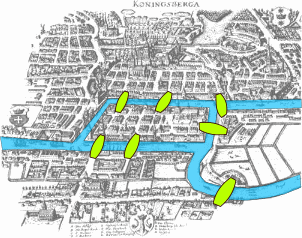
\includegraphics[width=\linewidth]{konigsberg_bridges}
    \caption{}\label{fig:konigsberg:map}
  \end{subfigure}
  \begin{subfigure}{.45\linewidth}
    \centering
    \begin{tikzpicture}
  [solmu/.style={circle,
    draw=black,
    inner sep=0pt,
    minimum size=7mm,
    node distance=5mm},
  spacer/.style={circle,
    minimum size=7mm,
    node distance=5mm}]
  \node[solmu](v1){};
  \node[spacer](s1)[right=of v1]{};
  \node[solmu](v2)[above=of s1]{};
  \node[solmu](v3)[below=of s1]{};
  \node[spacer](s2)[right=of s1]{};
  \node[solmu](v4)[right=of s2]{};
  \draw (v1) to [out=90, in=180] (v2);
  \draw (v1) to [out=10, in=270] (v2);
  \draw (v1) to (v4);
  \draw (v1) to [out=350, in=90] (v3);
  \draw (v1) to [out=270, in=180] (v3);
  \draw (v2) to (v4);
  \draw (v3) to (v4);
\end{tikzpicture}

    \caption{}\label{fig:konigsberg:tikz}
  \end{subfigure}
  \caption[Königsberg 1700-luvulla]{\subref{fig:konigsberg:map}) Königsberg 1700-luvulla, sillat vihreällä. \subref{fig:konigsberg:tikz}) Königsbergin sillat verkkona. Kuva \subref{fig:konigsberg:map}: Wikimedia Commons/Bogdan Giuşcă (CC BY-SA 3.0, \url{https://commons.wikimedia.org/wiki/File:Konigsberg_bridges.png}).}
  \label{fig:konigsberg}
\end{figure}

\section{Ongelman määrittely ja analyysi}
\label{sec:konigsberg_def}

Königbergin siltaongelma on seuraava:

\begin{problem}[Königsbergin siltaongelma]
  \label{prob:konigsberg}
  Onko Königsbergin kaupungissa sellaista kävelyreittiä, joka ylittää jokaisen sillan täsmälleen kerran. Joen ylittäminen muutoin kuin siltoja pitkin on kielletty. 
\end{problem}

\citet{euler36solutio} esitti ongelman abstraktina verkkoteorian ongelmana, missä saaret ja mantereet ovat solmuja ja sillat kaaria solmujen välillä (kuva~\ref{fig:konigsberg:tikz}). Hän osoitti, että ongelmaan ei ole ratkaisua. Nykytermein Königsbergin siltaongelman ratkaisu olisi \emph{Eulerin kulku} \engl{Euler(ian) path}, eli verkon polku joka kulkee jokaisen kaaren yli täsmälleen kerran. Eulerin tulos esitetään nykyään seuraavassa muodossa:

\begin{theorem}
  \label{thm:euler_path}
  Verkossa $G= (V, E)$ on Eulerin kulku jos ja vain jos verkossa on kaksi tai ei yhtään sellaista solmua, joiden aste on pariton.
\end{theorem}

Mikäli kulun täytyy palata takaisin alkusolmuun, puhutaan \emph{Eulerin kierroksesta}. Verkossa on Eulerin kierros jos ja vain jos siinä ei ole yhtään paritonasteista solmua.

\section{Eulerin kierroksen löytävä algoritmi}
\label{sec:euler_circuit_algo}

\citet{hierholzer73ueber} esitti tehokkaan algoritmin Eulerin kierron löytämiseksi. Algoritmi tekee mielivaltaisia kierroksia verkossa ja yhdistää niitä toisiinsa. Lopputulos tuottaa aina Eulerin kierroksen, sillä jokaisen solmun aste on aina parillinen. Algoritmi on esitetty pseudokoodina algoritmissa~\ref{alg:hierholzer}.

\begin{algorithm}[tb]
  \DontPrintSemicolon
  \SetKwInOut{Input}{syöte}\SetKwInOut{Output}{tulos}
  \SetKwProg{Fn}{function}{ }{end}
  \SetKwFunction{TeeKierros}{TeeKierros}
  \Input{Suuntaamaton verkko $G=(V, E)$ jonka jokaisen solmun aste on parillinen}
  \Output{Eulerin kierros $p$}
  \BlankLine
  $u \gets \text{mielivaltainen $V$:n solmu}$\;
  $(p, E') \gets $ \TeeKierros{$u, (V, E)$} \label{alg:hierholzer:kierrosi}\;
  \While{$E'\neq \emptyset$}{
    $u\gets \text{$p$:n mielivaltainen solmu jonka aste on $>1$ $E'$:ssa}$ \;
    $(q, E') \gets $ \TeeKierros{$u, (V, E')$} \;
    liitä polku $q$ polkuun $p$ \;
  }
  \Return{$p$}
  \BlankLine
  \Fn{TeeKierros(solmu $u$, kaaret $E$)}{
    $v\gets u$ \;
    $p\gets (u)$ \;
    \Repeat{$v = u$}{
      $w\gets \text{$v$:n mielivaltainen naapuri}$ \;
      poista kaari $\{v, w\}$ $E$:stä \;
      lisää solmu $w$ polkuun $p$ \;
      $v\gets w$ \;
    }
    \Return{$(p, E)$}
  }
  \caption{Hierholzerin algoritmi Eulerin kierroksen löytämiseksi.\label{alg:hierholzer}}
\end{algorithm}

Apufunktio \texttt{TeeKierros} tekee mielivaltaisen kierroksen alkaen solmusta $u$ ja käyttäen $E$:n kaaria. Tuloksena se palauttaa kierroksen $p$ ja kaarijoukon $E$ josta on poistettu $p$:n kaaret. Ensimmäinen kierros, rivillä~\ref{alg:hierholzer:kierrosi}, ei vielä välttämättä käytä kaikkia verkon kaaria. Niinpä apufunktiota kutsutaan toistuvasti satunnaisesta solmusta kunnes verkossa ei ole enää solmuja. 

Käyttämällä sopivia tietorakenteita, algoritmi~\ref{alg:hierholzer} voidaan toteuttaa lineaarisessa ajassa kaarten lukumäärän suhteen, $O(\abs{E})$.

% \texttt{ABCDEFGHIJKLMNOPQRSTUVWXYZÅÄÖ}\\
% \texttt{abcdefghijklmnopqrstuvwxyzåäö}\\
% \texttt{1234567890 .;-!?€}

% \textbf{\texttt{ABCDEFGHIJKLMNOPQRSTUVWXYZÅÄÖ}\\
% \texttt{abcdefghijklmnopqrstuvwxyzåäö}\\
% \texttt{1234567890 .;-!?€}}

% \setmonofont[StylisticSet=1]{Inconsolatazi4}
% \texttt{ABCDEFGHIJKLMNOPQRSTUVWXYZÅÄÖ}\\
% \texttt{abcdefghijklmnopqrstuvwxyzåäö}\\
% \texttt{1234567890 .;-!?€}

% \textbf{\texttt{ABCDEFGHIJKLMNOPQRSTUVWXYZÅÄÖ}\\
% \texttt{abcdefghijklmnopqrstuvwxyzåäö}\\
% \texttt{1234567890 .;-!?€}}


% Apufunktio \texttt{TeeKierros} tekee mielivaltaisen kierroksen alkaen solmusta $u$ ja käyttäen $E$:n kaaria.
